\documentclass[12pt]{article}
\usepackage{graphicx,import}
\usepackage{float}
\usepackage[svgnames]{xcolor} 
\usepackage{makecell}
\usepackage{fancyhdr}
\usepackage{subcaption}
\usepackage{hyperref}
\usepackage{enumitem}
\usepackage[many]{tcolorbox}
\usepackage{listings }
\usepackage[a4paper, total={6in, 8in} , bottom = 25mm , top = 25mm, headheight = 1.25cm , includehead,includefoot,heightrounded ]{geometry}
\usepackage{afterpage}
\usepackage{amssymb}
\usepackage{pdflscape}
\usepackage{gensymb}
\usepackage{textcomp}
\usepackage{tikz,pgfplots}
\usepackage{xecolor}
\usepackage{rotating}
\usepackage{pdfpages}
\usepackage[Kashida]{xepersian}
\usepackage[T1]{fontenc}
\usepackage{tikz}
\usepackage[utf8]{inputenc}
\usepackage{PTSerif} 
\usepackage{seqsplit}
\usepackage{hhline}
\usepackage{pgfgantt}
\usepackage{graphicx}
\usepackage{filecontents}
\usepackage{url} % for "\url" macro
\usepackage{babel}
\usepackage[backend=bibtex, style=numeric]{biblatex}

\addbibresource{refs.bib}

\graphicspath{ {./images/} }

\renewcommand\theadalign{bc}
\renewcommand\theadfont{\bfseries}
\renewcommand\theadgape{\Gape[4pt]}
\renewcommand\cellgape{\Gape[4pt]}

\usepackage[edges]{forest}

\usepackage{listings}
\usepackage{xcolor}

\hypersetup{
	colorlinks   = true, %Colours links instead of ugly boxes
	urlcolor     = blue, %Colour for external hyperlinks
	linkcolor    = blue, %Colour of internal links
	citecolor   = red %Colour of citations
}
 
\definecolor{codegreen}{rgb}{0,0.6,0}
\definecolor{codegray}{rgb}{0.5,0.5,0.5}
\definecolor{codepurple}{rgb}{0.58,0,0.82}
\definecolor{backcolour}{rgb}{0.95,0.95,0.92}
 
\NewDocumentCommand{\codeword}{v}{
\texttt{\textcolor{blue}{#1}}
}
\lstset{language=java,keywordstyle={\bfseries \color{blue}}}


\lstdefinestyle{mystyle}{
    backgroundcolor=\color{backcolour},   
    commentstyle=\color{codegreen},
    keywordstyle=\color{magenta},
    numberstyle=\tiny\color{codegray},
    stringstyle=\color{codepurple},
    basicstyle=\ttfamily\normalsize,
    breakatwhitespace=false,         
    breaklines=true,                 
    captionpos=b,                    
    keepspaces=true,                 
    numbers=left,                    
    numbersep=5pt,                  
    showspaces=false,                
    showstringspaces=false,
    showtabs=false,                  
    tabsize=2
}

\lstset{style=mystyle}

\settextfont[Scale=1.2, Path = fonts/ ,BoldFont={Bahij Nazanin-Bold} , ItalicFont = {IRNazaninIranic}]{Bahij Nazanin-Regular}
% \setlatintextfont[Scale = 1.0, Path = fonts/]{Garamond}
% \DefaultMathsDigits 
\DeclareMathSizes{11}{19}{13}{9} 
%\DeclareMathSizes{12}{14.4}{8}{9}





\newenvironment{changemargin}[2]{%
\begin{list}{}{%
\setlength{\topsep}{0pt}%
\setlength{\leftmargin}{#1}%
\setlength{\rightmargin}{#2}%
\setlength{\listparindent}{\parindent}%
\setlength{\itemindent}{\parindent}%
\setlength{\parsep}{\parskip}%
}%
\item[]}{\end{list}}


\definecolor{foldercolor}{RGB}{124,166,198}

\tikzset{pics/folder/.style={code={%
    \node[inner sep=0pt, minimum size=#1](-foldericon){};
    \node[folder style, inner sep=0pt, minimum width=0.3*#1, minimum height=0.6*#1, above right, xshift=0.05*#1] at (-foldericon.west){};
    \node[folder style, inner sep=0pt, minimum size=#1] at (-foldericon.center){};}
    },
    pics/folder/.default={20pt},
    folder style/.style={draw=foldercolor!80!black,top color=foldercolor!40,bottom color=foldercolor}
}

\forestset{is file/.style={edge path'/.expanded={%
        ([xshift=\forestregister{folder indent}]!u.parent anchor) |- (.child anchor)},
        inner sep=1pt},
    this folder size/.style={edge path'/.expanded={%
        ([xshift=\forestregister{folder indent}]!u.parent anchor) |- (.child anchor) pic[solid]{folder=#1}}, inner xsep=0.6*#1},
    folder tree indent/.style={before computing xy={l=#1}},
    folder icons/.style={folder, this folder size=#1, folder tree indent=3*#1},
    folder icons/.default={12pt},
}

\begin{document}


%%% title pages
\begin{titlepage}
\begin{center}
        
\vspace*{0.7cm}


\includegraphics[width=0.4\textwidth]{sharif1.png}\\
\vspace{0.5cm}
\textbf{ \Huge{\emph ‌آزمایشگاه سخت‌افزار} }\\
\vspace{0.5cm}
\textbf{ \Large{گزارش فاز سوم} }
\vspace{0.2cm}
       
 
      \large \textbf{دانشکده مهندسی کامپیوتر}\\\vspace{0.2cm}
    \large   دانشگاه صنعتی شریف\\\vspace{0.2cm}
       \large   ﻧﯿﻢ سال اول 02-01 \\\vspace{0.2cm}
      \noindent\rule[1ex]{\linewidth}{1pt}
استاد:\\
    \textbf{{جناب آقای دکتر اجلالی}}


دستیار آموزشی:\\
\textbf{{جناب آقای دکتر فصحتی}}

    \vspace{0.25cm}
    
    موضوع پروژه:\\
    
    \textbf{دید در شب اتومبیل}
    
    \vspace{0.35cm}
    
    
        شماره گروه:
    \textbf{{۶}}\\
    
اعضای گروه:\\

    \textbf{{علیرضا شاطری}}
    \\
   
     \textbf{{رضا امینی}}   
\end{center}
\end{titlepage}
%%% title pages


%%% header of pages
\newpage
\pagestyle{fancy}
\fancyhf{}
\fancyfoot{}
\cfoot{\thepage}
\chead{}
\rhead{
\includegraphics[width=0.1\textwidth]{sharif.png}}
\lhead{گزارش فاز سوم}
%%% header of pages

\newfontfamily\terminal{Courier New Bold}

\KashidaOff
 \newcommand{\inlineLatin}[1]{
	\small{\lr{{\terminal #1}}}
}


\tableofcontents
\listoffigures
\listoftables

\newpage
\section{مقدمه}

محصول نهایی این پروژه، یک سیستم دید در شب است که درون اتومبیل قرار می‌گیرد و به راننده هنگام رانندگی در تاریکی، کمک به سزایی می‌کند. در این سیستم اطلاعات از طریق یک دوربین حرارتی به ماژول رزپری منتقل می‌شود و کدهایی که در رزپبری قرار داده شده است با انجام پردازش تصویری ساده، تشخیص خواهد داد که آیا موجود زنده‌ای در میدان دید راننده حضور دارد یا خیر. همچنین از طریق چراغ و صدا نتیجه را به راننده اطلاع می‌دهد.
\\

در این فاز از پروژه ما باید بتوانیم یه طور عملی خروجی قابل استفاده از سنسور دما بگیریم تا در نهایت بتوانیم از خروجی آن استفاده کرده تا چراغ های اخطار را روشن کنیم.

\section{گزارش انجام پروژه}
\subsection{مشکل در روند پروژه}

ما در روز ارائه پروژه در فاز دوم دچار مشکل شدیم، متاسفانه کارت حافظه‌ی موجود در رزپبری پای خراب شد.

\subsubsection{فراهم سازی سخت افزار}

ما مجبور به خرید دوباره ی کارت حافظه شدیم و دوباره روند نصب سیستم عامل را طی کردیم، البته اشتباه سری قبل را تکرار نکردیم، در سری اول ما سیستم عامل قدیمی نصب کرده بودیم، در نتیجه ورژن پایتون آن کاملا قدیمی بود و در نصب یکسری کتابخانه دچار مشکل داشتیم، اما در این سری ورژن درستی از سیستم عامل ریزپبری را نصب کردیم که باعث شد رسیدن به خواسته ها سهل الوصول بشود.

\subsubsection{بازیابی کد}
با توجه به اینکه ما تمام کد های خود را در یک ریپازیتوری گیت نگهداری می‌کردیم در نتیجه به راحتی کد های خود را بازیابی کردیم و به حالت قبل از خرابی بازگشتیم.


\newpage

\subsection{اتصال سنسور دما}

\subsubsection{اتصال فیزیکی}

با توجه به گزارش قبلی ، سنسور دما را با استفاده از راهنمای زیر به رزپبری پای نصب کردیم.
\\
البته در این مرحله به مشکلات زیادی برخوردیم، زیرا نحوه اتصال به سنسور خیلی پایسته نبود و به راحتی دچار مشکل می‌شد، برای رفع این مشکل ما مجبور به استفاده از سیم هایی غیر از سیم های نر نر یا نر ماده شدیم تا بتوانیم اتصال پایدار تری با سنسور داشته باشیم.

\begin{figure}[h]
	\begin{center}
		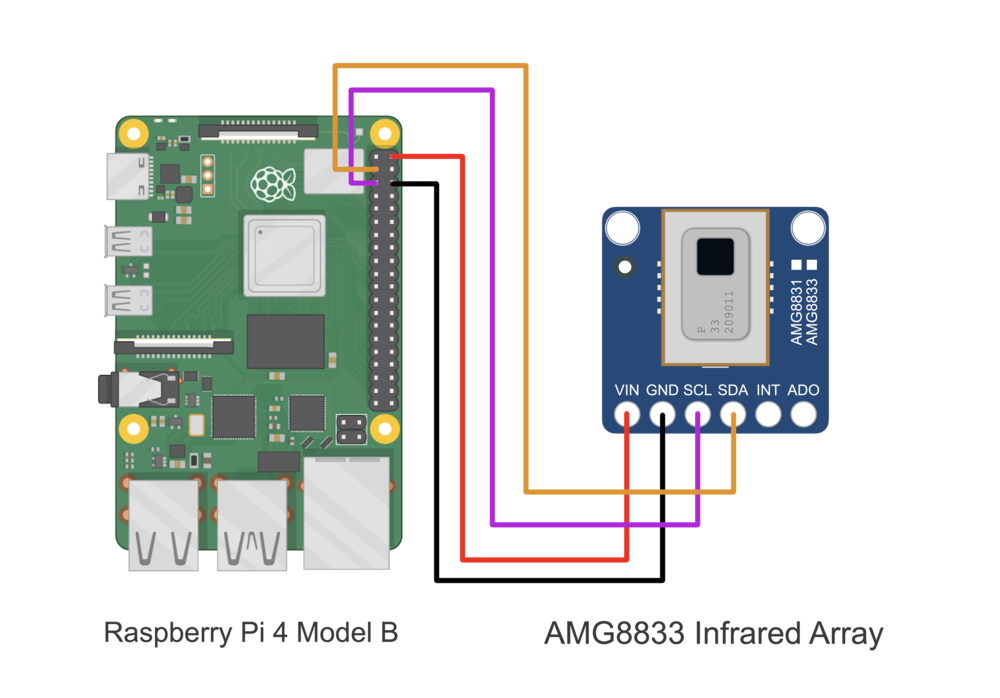
\includegraphics[width=.75\textwidth]{images/amg8833_RPi4_wiring.png}
	\end{center}
	\caption{راهنمای نصب سنسور دما}
\end{figure}

\subsubsection{پیاده سازی کد}

برای پیاده سازی کد از یک کد آماده استفاده کردیم که به صورت زنده ورودی های سنسور را نمایش میداد، ما برای دریافت اینسایت و فهم بیشتر از ورودی های سنسور با کتابخانه \lr{pandas} ورودی را به نمایش گذاشتیم.
 
\\
 
 با تجوه به شکل زیر که خروجی ما می‌باشد می‌توان فهمید که در قسمت هایی که قسمتی از بدن انسان وجود دارد دما در بازه‌ی ۳۰ تا ۴۰ درجه قرار میگیرد که با استفاده از آن می‌توان تشخیص داد که آیا انسانی وجود دارد یا خیر.

\\
 
\begin{figure}[h]
	\begin{center}
		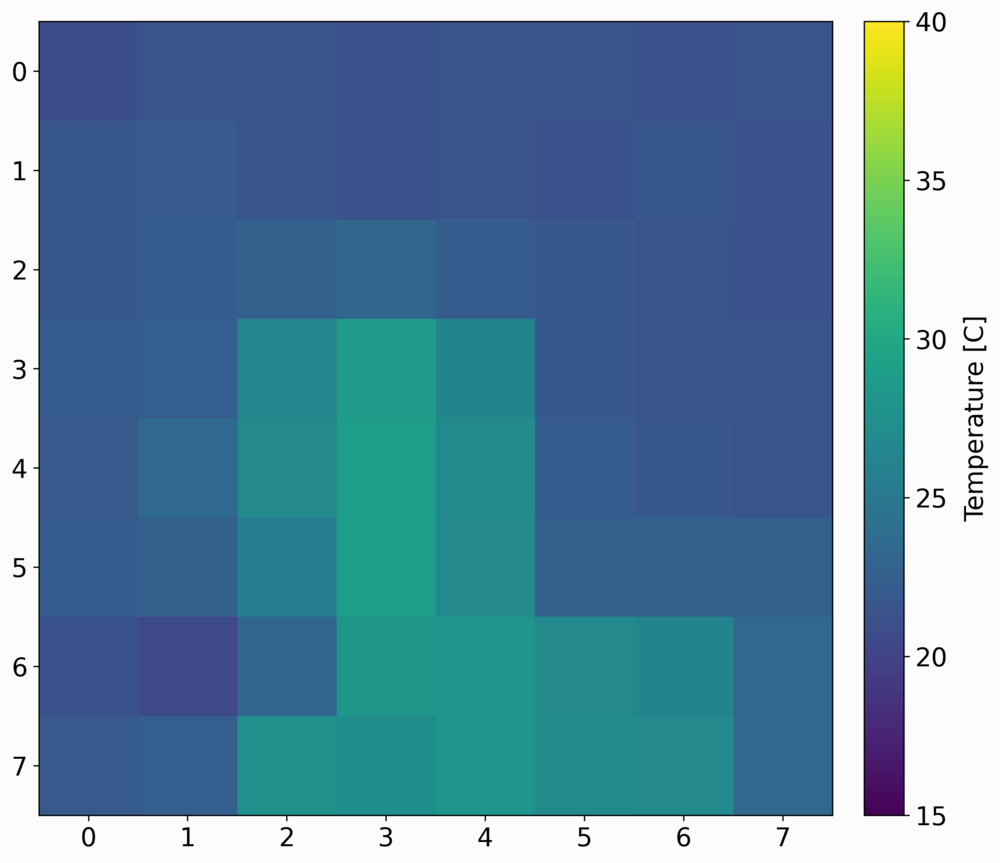
\includegraphics[width=.75\textwidth]{images/AMG8833_IR_cam_test.png}
	\end{center}
	\caption{خروجی سنسور دما}
\end{figure}

\newpage

\section{قدم آخر}

در قدم بعدی باید جایگاه انسان در قسمت چپ یا راست جاده تشیخص داد و آن را در چراغ های اخطار نشان داد، و بعد از آن پروژه به اتمام می‌رسد.
\end{document}

